\documentclass{article}

\usepackage{czt}
\usepackage{geometry}
\geometry{a4paper, portrait, margin=2cm}

\usepackage{fancyhdr}
\pagestyle{fancy}
\lhead{Formal Specification - Mairead  Meagher}
\rhead{Anton Krug - 20062210}
\rfoot{Page \thepage}
\cfoot{}
\renewcommand{\headrulewidth}{0pt}

%got tired of typing and copy pasting so made command for cases where the new state is the same as the previous state
\newcommand{\same}[1]{\\{#1}'={#1}}

%the supersets will never change, DRY, just lazy to type them every time
\newcommand{\sameObvious}[1]{\same{rooms}\same{allThings}\same{noiseThings}\same{tempThings}\same{lightThings}\same{actuatorThings}  }

\usepackage[document]{ragged2e}

\usepackage{graphicx}

%\usepackage{hyperref}

%\usepackage{tgbonum}

%\usepackage[none]{hyphenat}

\newcommand\invisiblesection[1]{%
  \refstepcounter{section}%
  \addcontentsline{toc}{section}{\protect\numberline{\thesection}#1}%
  \sectionmark{#1}}

\begin{document}

\pagestyle{empty}

 
\center
{\Huge Formal specification -  Z spec assignment}

\begin{figure}[h!]
	
\includegraphics[width=\textwidth]{images/hammer.png}
    \label{fig:modules}
\end{figure}

{\Huge Pancake - IoT framework }\\

{\huge Anton Krug - 20062210
\vfill
}







\newpage
\pagestyle{fancy}
\tableofcontents






\newpage
\section{Introduction}

\justify
There is a considerable amount of available Internet Of Things (IoT) and home automation technologies. Some are proprietary and some are open source, but it’s rare to offer full freedom and extensibility by design on very low-cost devices while providing ready-to-use products. Pancake framework should focus on this gap and offer very low cost and open devices based on ESP8266 chips. Services could prepared for home automation purpose and but the flexibility allows many other uses cases. These goals can be achievable thanks to modern languages and frameworks such as nodeJS and EcmaScript7. Public swagger API specification for Clashmore module could offer shallow learning curve for manufacturers creating compatible devices or offer  iOS/Android UI for Clashmore thanks to Swagger auto generators. Pancake Service should offer SDK which will allow 3rd party developers writing universal and portable apps for any use cases easily. In the future, this could lead to extensions, an app marketplace and own ecosystem. Pancake Service SDK will be distributed as an npm package only, but in the future 3rd parties could offer iOS/Android SDKs as well. Good end-user adoption could be achieved by offering the Pancake Service as cloud service and as downloadable container for these who would prefer to host it locally. This architecture should allow pleasant experience and many possibilities for the end-user. The app developer can be independent from end-user and independent from the device manufacturer as well.\\

Security is a significant aspect of this project because embedded devices tend to be involved in many attacks. They often are low on resources and low on entropy. Some devices might have hardware random generators, but many embedded devices have resort to flawed pseudo random generators. 
 
\begin{itemize}
  \item Devices can be used against the owner because they are capable to actuate physical  real-world objects. 
  \item Devices can be used as a swarm in a distributed denial of service attack against remote target.
\end{itemize}

\begin{figure}[h!]
	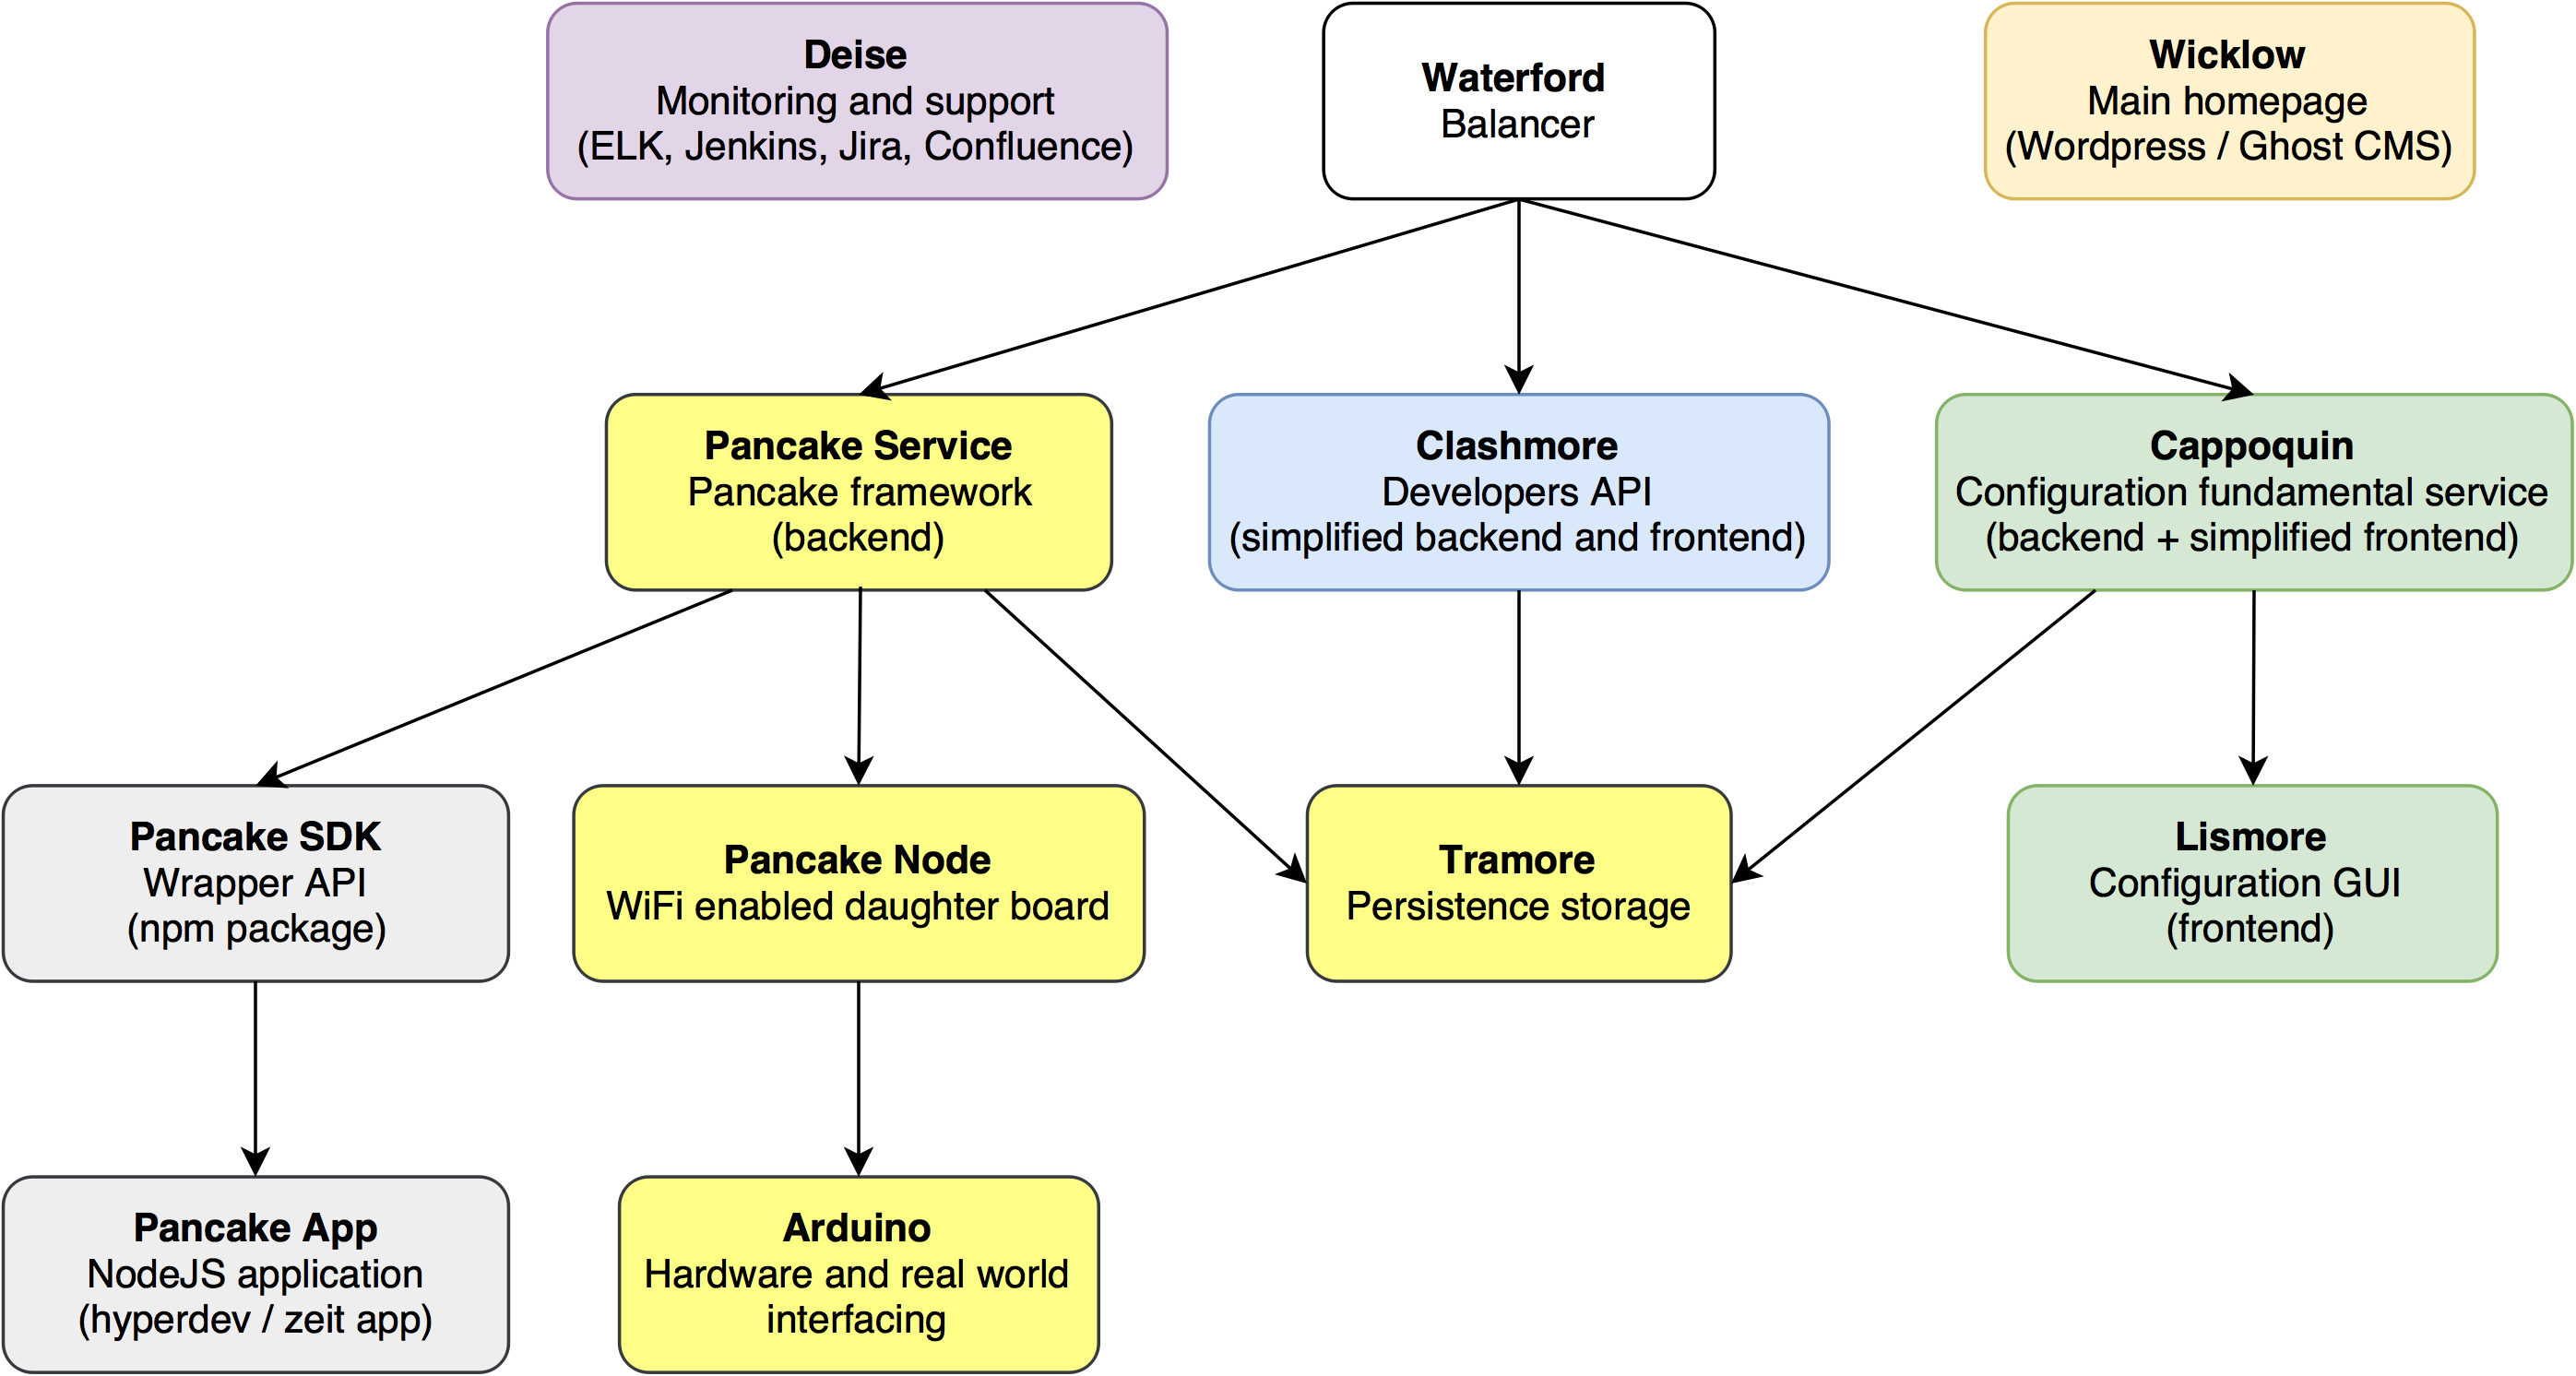
\includegraphics[scale=0.168]{images/modules.png}
    \caption{All modules involved in the Pancake project}
    \label{fig:modules}
\end{figure}


Because of large scale and scope of this project as shown in the figure \ref{fig:modules}, for the formal specification I will only focus specifying a simplified subset of the project and describe only Pancake Service and Pancake Platform. PancakeService which consists of multiple instances of PancakePlaforms. Each platform is containing all the required Things and their connection between each other. Many of the Things are only sensors to sense the environment while some can be actuators altering the real world.










\newpage
\section{Global types and variables}

\begin{zed}
  [ CHAR ] \\
  [ ROOM ]  \\
  [ LOCATION ]  \\
  [ TIME ]  
\end{zed}

\begin{axdef}
 times: \iseq TIME
\end{axdef}

\begin {axdef}
 BOOLEAN::= true / false
\end{axdef}

\begin {axdef}
  toLower: CHAR \fun CHAR
\where
  toLower = \{ \\
  \indent `A` \mapsto `a`, `B` \mapsto `b`, `C` \mapsto `c`, \\
  \indent `a` \mapsto `a`, `b` \mapsto `b`, `c` \mapsto `c`, \\
  \indent `0` \mapsto `0`, `1` \mapsto `1`, `2` \mapsto `2`, \\
  \indent `$@$` \mapsto `$@$`, `.` \mapsto `.`, `\_` \mapsto `\_` ... \} 
\end{axdef}


\begin {axdef}
  charAlpha: \power CHAR
\where
  charAlpha = \{ `a` ... `z` , `A` ... `Z` \} 
\end{axdef}


\begin {axdef}
  charNum: \power CHAR
\where
  charNum = \{ `0` ... `9`  \} 
\end{axdef}








\newpage
\section{Pancake Platform}
\subsection{PancakePlatform schema}

\label{toc:PancakePlatform}
\begin{schema}{PancakePlatform}
  rooms: \power ROOM \\
  roomLocations: LOCATION \pfun ROOM \\
  things: THING \pfun LOCATION \\
  allThings: \power THING \\
  noiseThings, tempThings, lightThings, actuatorThings: \power THING \\
  thingNames: THING \pfun \seq CHAR\\
  minimums: THING \pfun \num \\
  thresholds: THING \pfun \num \\
  maximums: THING \pfun \num \\
  data: THING \pfun \seq \num \\
  edges: THING \fun \seq THING
\where
  < noiseThings, tempThings, lightTHings, actuatorThings> \partition allThings \\\\
  
  \dom edges \in allThings \setminus actuatorThings\\
  \ran edges \in actuatorThings\\\\

  \forall thing: \dom data | thing \in actuatorThings @ \\
	  \indent minimums(thing) \leq thresholds(thing)  \leq maximums(thing) \\  \\

  \forall thing: \dom data @ \\
	  \indent  ( 30 > \# thingNames(thing) > 3 ) \land \\
	  \indent ( \forall index: dom(data(thing)) @ minimums(thing) \leq data(thing)(index) \leq maximums(thing) ) \\  \\

   \forall source: \dom edges \\
	   \indent \forall destination: edges(source) @  data(destination) = data(source) \land \#data(source) > 0 \\\\
	   
	\dom thingNames = \dom minimums = \dom maximums = \dom things

\end{schema}
This is most important schema of the whole project, contains all the Things and keeps all their settings, connections between  and history data. The thing could a physical sensor with internet connection implemented in hardware with ESP 2866 capable of sending data to the platform over WiFi. Depending what the Thing can do or what type it is they are split between consumers called actuators and between producers which sense real-life physical values as numbers and stored inside data set. If there is an entry in thingNames there is a guarantee that there is mapping in minimus and maximums as well. 


\begin{itemize}
  \item rooms contain all possible rooms in the system.
  \item roomLocations maps multiple specific locations inside the room.
  \item things are maped with their location inside the room.
  \item allThings contains all possible things in the system and is partitioned betwen noise, temperature, light and actuator Things.
  \item each Thing in the system has:
	\begin{itemize}
   		\item thingName a string with minimum lenght of 4 and maximum of 29.
   		\item minimum, maximum range constrains which limit the data inside these boundaries.
   		\item Their history data which logs all their value over time.
	\end{itemize}
  \item Actuators on top of all the above properties has threshold information as well, but do not have mapping for edges. They can't connect any further Thing, because they are consuming the data and not passing it through.
  \item While non-actuators have list of edges containing information to what actuator things they are connected to. Edges can connect only to actuators things and they will share the same history data with connected Thing.
  
\end{itemize}




\newpage
\subsection{Operations}

\label{toc:InitPancakePlatform}
\subsubsection{InitPancakePlatform}
\begin{schema}{InitPancakePlatform}
  PancakePlatform'
\where
  roomLocations = < > \\
  things = < > \\
  thingNames = < > \\
  minimums = <> \\
  thresholds = <> \\
  maximums = <> \\
  data =  < > \\
  edges =  < > \\
\end{schema}
InitPancakePlatform will initialise platform for the very first time with empty data


\label{toc:AddLocation}
\subsubsection{AddLocation}
\begin{schema}{AddLocation}
  \Delta PancakePlatform \\
  room?: ROOM \\
  location?: LOCATION
\where
  location \notin \dom roomLocations \\
  roomLocations' = roomLocations \cup \{ location? \mapsto room? \} \\

  \same{things}
  \same{thingNames}
  \same{minimums}
  \same{thresholds}
  \same{maximums}
  \same{data}
  \same{edges}
  \sameObvious{}
\end{schema}
A room can contain multiple specific locations where the things could be placed, but location needs to be unique for each thing. All other information in the system will not change.


\newpage
\label{toc:RemoveLocation}
\subsubsection{RemoveLocation}
\begin{schema}{RemoveLocation}
  \Delta PancakePlatform \\
  location?: LOCATION
\where
  location \in \dom roomLocations \\
  location \notin \ran things \\
  roomLocations' = \{ location? \} \ndres roomLocations \\ 
  
  \same{things}
  \same{thingNames}
  \same{minimums}
  \same{thresholds}
  \same{maximums}
  \same{data}
  \same{edges}
  \sameObvious{}
\end{schema}
RemoveLocation operation will remove only locations which are not yet associated with the thing. If there is already mapping made, you need to call RemoveThing from chapter \ref{toc:RemoveThing} first. All other information in the system will not change.

\newpage
\label{toc:AddThing}
\subsubsection{AddThing}
\begin{schema}{AddThing}
  \Delta PancakePlatform \\
  thing?: THING \\
  location?: LOCATION \\
  name?: seq CHAR \\
  min?: \num \\
  max?: \num
\where
  30 > \# name? > 3 \\
  thing? \notin actuatorThings \\
  thing? \notin \dom thingNames \\
  location? \in \dom roomLocations \\
  location? \notin \ran things \\
  thingNames'=thingNames \cup \{ thing? \mapsto  name?  \} \\ 
  things' = things \cup \{ thing? \mapsto location? \}
  minimums' = minimus \cup \{ thing? \mapsto min? \} \\
  maximus' = maximus \cup \{ thing? \mapsto min? \} \\
  edges' = edges \cup \{ thing? \mapsto <> \}  \\


  \same{roomLocations}
  \same{thresholds}
  \same{data}
  \sameObvious{}

\end{schema}
AddThing will append given thing, the call needs to be given the Thing itself, it's name, minimum and maximum ranges. Location needs to be unique, associated with a room, but not with any previous Thing. The thing can't be actuatorThing (for actuators there is call called  AddActuatorThing). The name needs to be more than 3 characters and less than 30, The thing can't be in the system already. After all, requirements are meet, the platform will be updated with new thingName, minimums, maximums and empty sequence  of edges associated with this Thing. All other information will stay same.

\newpage
\label{toc:AddActuatorThing}
\subsubsection{AddActuatorThing}
\begin{schema}{AddActuatorThing}
  \Delta PancakePlatform \\
  thing?: THING \\
  location?: LOCATION \\
  name?: seq CHAR \\
  min?: \num \\
  max?: \num \\
  threshold?: \num 
\where
  30 > \# name? > 3 \\
  thing? \in actuatorThings \\
  thing? \notin \dom thingNames \\
  location? \in \dom roomLocations \\
  location? \notin \ran things \\  
  things' = things \cup \{ thing? \mapsto location? \} \\
  min? \leq threshold? \leq max? \\
  thingNames'=thingNames \cat < name? > \\ 
  minimums' = minimus \cat < min? > \} \\
  thresholds' = thresholds \cat < threshold? >  \\
  maximus' = maximus \cat < min? > \\
  edges' = edges \cup \{ thing? \mapsto \emptyset \}  \\

  
  \same{roomLocations}
  \same{data}
  \sameObvious{}
  
\end{schema}
AddActuatorThing will append a given thing, the call needs to be given the Thing itself, it's name, minimum and maximum ranges. Location needs to be unique, associated with a room, but not with any previous Thing. The thing needs to be actuatorThing (for non-actuators there is call called  AddThing). The name needs to be more than 3 characters and less than 30, The thing can't be in the system already. After all, requirements are meet, the platform will be updated with new thingName, minimums, maximums and empty sequence  of edges associated with this Thing. All other information will stay same.




\newpage
\label{toc:AddData}
\subsubsection{AddData}
\begin{schema}{AddData}
  \Delta PancakePlatform \\
  thing?: THING \\
  time?: TIME \\
  value?: \num
\where
  thing? \in \dom thingNames \\
  thing? \notin actuatorThings\\
  time? \in times \\
  minimums(thing?) \leq value? \leq maximums(thing?) \\
  data' = data \oplus \{ thing? \mapsto (time? \mapsto value?) \}\\

  \same{roomLocations}
  \same{things}
  \same{thingNames}
  \same{minimums}
  \same{thresholds}
  \same{maximums}
  \same{edges}
  \sameObvious{}
 
\end{schema}
AddData is called when a given Thing wants to store the value it measured. It is checked if the thing is in Platform and if the time is valid. The data value needs to be within the minimum and maximum ranges. All other information will stay the same. The data can be entered into the Platform only from non-Actuator Things. All other information will stay same.

\newpage
\label{toc:RemoveThing}
\subsubsection{RemoveThing}
\begin{schema}{RemoveThing}
  \Delta PancakePlatform \\
  thing?: THING
\where
  thing? \in \dom thingNames \\
  
  thingNames' = \{  thing? \}  \ndres thingNames \\
  things' = \{  thing? \}  \ndres thingNames \\  
  minimus' = \{  thing? \}  \ndres minimus \\
  thresholds' = \{  thing? \}  \ndres thresholds \\
  maximus' = \{  thing? \}  \ndres maximus \\
  data' = \{  thing? \}  \ndres data \\
  edges' = \{  thing? \}  \ndres edges \\
  
  \same{roomLocations}
  \same{thingNames}
  \same{minimums}
  \same{thresholds}
  \same{maximums}
  \same{data}
  \same{edges}
  \sameObvious{}  
\end{schema}
RemoveThing requires only thing parameter and successfully removes it's mapping from thingNames, minimus, thresholds, maximums, data and edges. Will work with both non-actuator things and actuator things, but they need to be already in the system and have stored thingName, which will ensure that they have stored minimums, maximums as well. All other information will stay same.

\newpage
\label{toc:ChangeThingRange}
\subsubsection{ChangeThingRange}
\begin{schema}{ChangeThingRange}
  \Delta PancakePlatform \\
  thing?: THING \\
  min?: \num  \\
  max?: \num
\where
  thing? \in \dom thingNames \\
  thing? \notin actuatorThings\\
  data' = \{ thing? \} \ndres data\\

  data' = data \oplus  \{ thing? \mapsto <> \} \\
  minimus' = minimus \oplus  \{ thing? \mapsto min? \}  \\
  maximus' = maximus \oplus \{ thing? \mapsto max? \} \\

  \same{roomLocations}
  \same{things}
  \same{thingNames}
  \same{thresholds}
  \same{edges}
  \sameObvious{}
\end{schema}
If the Thing was setup with wrong range and needs to be updated in the runtime then, ChangeThingRange can be called. It will require desired Thing and the new min and max values. The thing needs to be inside the system already and can't be used with actuatorThings (for these there is ChangeActuatorThingRange operation). The data for the thing needs to be cleared because the new range could invalidate the constrain of the existing data and probably this is the reason why the range needs to be updated. 

\newpage
\label{toc:ChangeActuatorThingRange}
\subsubsection{ChangeActuatorThingRange}
\begin{schema}{ChangeActuatorThingRange}
  \Delta PancakePlatform \\
  thing?: THING \\
  min?: \num  \\
  threshold?: \num  \\
  max?: \num
\where
  thing? \in \dom thingNames \\
  thing? \in actuatorThings\\
  data' = data \oplus  \{ thing? \mapsto <> \} \\
  minimus' = minimus \oplus  \{ thing? \mapsto min? \} \\
  thresholds' = thresholds \oplus \{ thing? \mapsto threshold? \}  \\
  maximus' = maximus \oplus \{ thing? \mapsto max? \} \\

  \same{roomLocations}
  \same{things}
  \same{thingNames}
  \same{edges}
  \sameObvious{}
\end{schema}
If an actuator Thing was setup with wrong range and needs to be updated in the runtime, then ChangeThingRange can be called. It will require desired Thing and the new min and max values. The thing needs to be inside the system already and can't be used with non-actuatorThings (for these there is ChangeThingRange operation). The data for the thing needs to be cleared because the new range could invalidate the constrain of the existing data and probably this is the reason why the range needs to be updated. 


\label{toc:FindWhen}
\subsubsection{FindWhen}
\begin{schema}{FindWhen}
  \Xi PancakePlatform \\
  thing?: THING \\
  val?: \num \\
  when!: \iseq TIME
\where
  thing? \in \dom data \\
  when!= times \limg data( thing? ) \inv \limg val? \rimg \rimg
\end{schema}
To find all moments when the thing's data had specified value a FindWhen operation can be called. It doesn't change anything in the platform, only returns data. It will return a sequence of all times when the specific val was recorded. The thing needs to be in the system.


\newpage
\label{toc:AddEdge}
\subsubsection{AddEdge}
\begin{schema}{AddEdge}
  \Delta PancakePlatform \\
  source?: THING \\
  destination?: THING
\where
  source? \in \dom thingNames \\
  destination? \in \dom thingNames \\
  source? \notin actuatorThings \\
  destination? \in actuatorThings \\
  \forall s:THING | s \in allThings \land s \notin actuatorThings @  destination? \notin edges(s?) \\
  edges' = edges \oplus \{ edges(source?) \cat < destination? > \}  \\

  \same{roomLocations}
  \same{things}
  \same{thingNames}
  \same{minimums}
  \same{thresholds}
  \same{maximums}
  \same{data}
  \sameObvious{}

\end{schema}
Operation AddEdge is used to add to a non-actuator source thing an edge connection which is pointing to an actuator destination thing.  Both source and destination things needs to be part of the system and the destination thing cannot be used as a destination edge by any other non-actuator things. Only one non-actuator thing can point to the actuator thing in the whole system. The operation will update the edges, but all other information will stay same.

\newpage
\label{toc:RemoveEdge}
\subsubsection{RemoveEdge}
\begin{schema}{RemoveEdge}
  \Delta PancakePlatform \\
  source?: THING \\
  destination?: THING
\where
  source? \in \dom thingNames \\
  destination? \in \dom thingNames \\
  source? \notin actuatorThings \\
  destination? \in actuatorThings \\
  destination? \notin edges(source?) \\
  edges' = edges \oplus squash(edges(source?) \nrres \{ destination? \}  ) \\


  \same{roomLocations}
  \same{things}
  \same{thingNames}
  \same{minimums}
  \same{thresholds}
  \same{maximums}
  \same{data}
  \sameObvious{}
\end{schema}
A RemoveEdge operation is useful to make sure a given source non-actuator thing is not using destination actuator thing as an edge. Both source and destination things needs to be part of the system. The operation will update the edges, but all other information will stay same.


\label{toc:GetThingStats}
\subsubsection{GetThingStats}
\begin{schema}{GetThingStats}
  \Xi PancakePlatform \\
  thing?: THING \\
  timeStart?: TIME \\
  timeEnd?: TIME \\
  min!: \num \\
  avg!: \num  \\
  med!: \num \\
  max!: \num \\ 
\where
  \{ timeStart?, timeEnd? \} \subseteq times \\
  times\inv(timeStart?) < times\inv(timeEnd?) \\
  thing? \in \dom(data) \\
  \exists samples: \seq \num @  samples = squash( times\inv(timeStart?) ... times\inv(timeEnd?) \dres data(thing?) )  \\
  min! = minimum(samples)
  avg! = mean(samples) \\
  med! = median(samples) \\
  max! = maximum(samples) \\
\end{schema}
Statistical information  can be gained with GetThingStats operation. It will not change anything in the platform, only return requested, min,max, avg and med results. The given parameter thing needs to be part of the system and the timeStart and timeEnd needs to be valid times and timeStart needs happen before the timeEnd. The operation is using the mathematical functions from chapter \ref{math:maximum} to compute the statistical results on data which was stored between given time interval.


\newpage
\label{toc:isThingOver}
\subsubsection{isThingOver}
\begin{schema}{isThingOver}
  \Xi PancakePlatform \\
  thing?: THING \\
  result!: BOOLEAN 
\where
  time? \in times \\
  thing? \in \dom(data) \\  
  thing? \in actuatorThings \\
  \#data(thing?) > 0 \\
  ( data(thing?)(\#data(thing?)) > thresholds(thing?) \land result! = true ) \lor \\
  ( data(thing?)(\#data(thing?)) \leq thresholds(thing?) \land result! = false ) 
\end{schema}
Use isThingOver operation to find out if given actuator thing is over the threshold. Operation requires the thing to have some data and it will return the state based on the very last data entry. And it will return BOOLEAN response if the thing at that time was over the threshold. Operation itself will not affect any information inside the platform.




\label{toc:isThingUnder}
\subsubsection{isThingUnder}
\begin{schema}{isThingUnder}
  \Xi PancakePlatform \\
  thing?: THING \\
  result!: BOOLEAN 
\where
  time? \in times \\
  thing? \in \dom(data) \\  
  thing? \in actuatorThings \\
  \#data(thing?) > 0 \\
  ( data(thing?)(\#data(thing?)) \leq thresholds(thing?) \land result! = true ) \lor \\
  ( data(thing?)(\#data(thing?)) > thresholds(thing?) \land result! = false ) 
\end{schema}
Use isThingUnder operation to find out if given actuator thing is below, or at the threshold. Operation requires valid time when we the actuator was over the threshold, know the specific thing. And it will return BOOLEAN response if the thing at that time was below the threshold. Operation itself will not affect the state of the platform.





\newpage
\section{PancakeService}
\subsection{Schemas}

\label{toc:Customer}
\subsubsection{Customer}
\begin{schema}{Customer}
  name: \seq CHAR\\
  email: \seq CHAR\\
  password: \seq CHAR
\where
  70 \ge \# name \geq 2 \\
  70 \ge \# email  \geq 5 \\
  \exists_1 char:CHAR | char \in \ran email @ char=`$@$` \\
  \exists char:CHAR | char \in \ran email @ char=`$.$` \\
  100 \ge \# password \geq 10 \\
  \exists char:CHAR | char \in \ran password @ char \in charAlpha  \\
  \exists char:CHAR | char \in \ran password @ char \in charNum  \\
\end{schema}
A Customer has stored his name and credentials, the name needs to be longer than 1 character and shorter than 71. Email needs to be at least 5 characters long and up to 70, 5 characters is the absolute minimum for email format `a@b.c`, the email needs to contain one `@` character and at least one dot. The password needs to be longer than 9 and less than 101 while they needs to use at least one alphanumerical character and one numerical character.


\label{toc:PancakeService}
\subsubsection{PancakeService}
\begin{schema}{PancakeService}
  customers: \seq Customer \\
  platforms: \seq PancakePlatform 
\where
  \#customers = \# platforms
\end{schema}
PancakeService holds all the customers and all their individual instances of their platforms. Both customers and platforms needs to be the same size.







\newpage
\subsection{Operations}


\label{toc:InitPancakeService}
\subsubsection{InitPancakeService}
\begin{schema}{InitPancakeService}
  PancakeService'
\where
 customers = < > \\
 platforms = < >
\end{schema}
InitPancakeService operation will initialize empty sequences for customers and platforms.

\label{toc:RegisterCustomer}
\subsubsection{RegisterCustomer}
\begin{schema}{RegisterCustomer}
  \Delta PancakeService \\
  newCustomer?: Customer \\
  emptyPlatform: PancakePlatform
\where
  newCustomer \notin customers \\
  customers' = customers \cup newCustomer \\
  platforms' = platforms \cup emptyPlatform 
\end{schema}
To add new customer a RegisterCustomer operation can be used. A newCustomer and emptyPlatform needs to be supplied. An existing customer can't register again. If desired customers can create a new customer account under a different email.


\label{toc:RegisteredCustomers}
\subsubsection{RegisteredCustomers}
\begin{schema}{RegisteredCustomers}
  \Xi PancakeService \\
  count!: \nat
\where
  count! = \# \dom customers
\end{schema}
To find out how popular the Pancake is there is simple operation RegisteredCustomers. It will count how many existing customers the PancakeService has. The operation doesn't change any information in the service.

\newpage
\label{toc:LoginCustomer}
\subsubsection{LoginCustomer}
\begin{schema}{LoginCustomer}
  \Xi PancakeService \\
  email?: \seq CHAR \\
  password?: \seq CHAR\\
  logged!: BOOLEAN
\where
  70 \ge \# email?  \geq 5 \\
  \exists_1 char:CHAR | char \in \ran email? @ char=`$@$` \\
  \exists char:CHAR | char \in \ran email? @ char=`$.$` \\
  100 \ge \# password? \geq 10 \\
  \exists char:CHAR | char \in \ran password? @ char \in charAlpha  \\ 
  \exists char:CHAR | char \in \ran password? @ char \in charNum  \\ \\
  
  \exists e: \seq CHAR | e =  email? \comp toLower  \\ \\
  ( \exists_1 c:Customer |  c \in customers  \land c.email = e \land c.password = password? @ logged! = true ) \\
  \indent \indent \indent \lor \\
  ( \not \exists c:Customer |  c \in customers  \land c.email = e \land c.password =  password? @ logged!=false)
\end{schema}
To authenticate existing customer a LoginCustomer operation can be called. Email needs to be at least 5 characters long and up to 70, 5 characters is an absolute minimum for email format `a@b.c`, the email needs to contain one `@` character and at least one dot. The password needs to be longer than 9 and less than 101 while they needs to use at least one alphanumerical character and one numerical character. The email then will be converted to a lowCaps string. The operation will not change any state, only verify if there exists any customer who has same email and password, if yes it will return BOOLEAN true for logged. If there will be no single entry where email and password were matched it will return false. 


\label{toc:GetCustomersPlatform}
\subsubsection{GetCustomersPlatform}
\begin{schema}{GetCustomersPlatform}
  \Xi PancakeService \\
  loggedCustomer?: Customer \\
  platform!: PancakePlatform
\where
  loggedCustomer \in customers \\
  
  platform! = platforms( customers\inv(customer))
\end{schema}
Each customer has an own dedicated platform, use GetCustomersPlatform operation to find what platform is allocated to the loggedCustomer. Platform state is not modified, loggedCustomer is provided and returned platform.



\label{toc:DeleteCustomer}
\subsubsection{DeleteCustomer}
\begin{schema}{DeleteCustomer}
  \Delta PancakeService \\
  customerToDelete?: Customer
\where
  customerToDelete \in customers \\
  customers' = squash( customers \nrres \{ customerToDelete \} )\\
  platforms' = squash(  customers\inv(customerToDelete) \ndres platforms) \\
\end{schema}
To unsubscribe from the service DeleteCustomer operation can be used with customerToDelete argument. 


\newpage
\label{toc:ChangePassword}
\subsubsection{ChangePassword}
\begin{schema}{ChangePassword}
  \Delta PancakeService \\
  customer?: Customer \\
  customerWithNewPassword?: Customer
\where
  customer \in customers \\  
  customers' = customers \oplus  \{ customers \inv \limg \{ customer? \} \rimg  \mapsto customerWithNewPassword? \}  \\
  platforms' = platforms 
\end{schema}
Operation ChangePassword requires customer and the same customer with updated new password. It will interchange the customer with the customerWithNewPassword inside the customers, while platforms will stay untouched.






\newpage
\section{Functions}

\subsection{sum}
\label{math:sum}
\begin {axdef}
 sum: \seq X \fun \num
\where
 \forall s: \seq X; x: \num @ \\
  sum < > = 0 \land \\
  sum <H> \cat T =  H + sum(T)  
\end{axdef}
The sum will split the sequence into head and tail and recursively calculate sum of all members  of the sequence.

\subsection{mean}
\label{math:mean}
\begin {axdef}
 mean: \seq_1 \num \fun \num
\where
 \forall sequence: \seq_1 \num @ mean(sequence) = sum(sequence) \div \#sequence
\end{axdef}
Mean will calculate the average from the sequence of the data by summing up the whole sequence and then diving by the size of the sequence.

\subsection{median}
\label{math:median}
\begin {axdef}
 median: \seq_1 \num \fun \num
\where
 \forall sequence: \seq_1 \num @ \\

  \indent \exists_1 Historygram: \num \pfun \nat_1 @ \\
  	\indent \indent \dom(Historygram) = \ran(sequence) \land \\
  	\indent \indent ( \forall index:\dom(Historygram) @ Historygram(index) = \# (sequence \rres\{index\}) ) \land \\
  	\indent \indent  \exists_1 median(sequence): \num | median(sequence) \in \dom(Historygram) @ \\
	  	\indent \indent \indent Historygram(median(sequence)) = max( \ran Historygram ) 

\end{axdef}
Median is calculated with help of histogram. First the function will map how often each value was used, then it will find the value of the most used one.

\subsection{maximum}
\label{math:maximum}
\begin {axdef}
 maximum: \seq_1 \num \fun \num
\where
 \forall sequence: \seq_1 \num @  maximum(sequence) = max( \ran sequence)
\end{axdef}
The maximum is a simple function which calculates the maximum value from the range of the given sequence.

\subsection{minimum}
\label{math:minimum}
\begin {axdef}
 minimum: \seq_1 \num \fun \num
\where
 \forall sequence: \seq_1 \num @  minimum(sequence) = min( \ran sequence)
\end{axdef}
Minimum is a simple function which calculates the minimum value from the range of the given sequence.


\end{document}

